\documentclass[tikz,border=5mm]{standalone}
\usepackage{tikz}
\usetikzlibrary{arrows.meta, positioning, shapes.geometric, calc, backgrounds, fit, matrix, patterns, decorations.pathmorphing, shadows}

% --- COLOR DEFINITIONS ---
\definecolor{Garnet}{HTML}{73000A}
\definecolor{CSecondaryRed}{HTML}{CC2E40}
\definecolor{CBlue}{HTML}{466A9F}
\definecolor{CDark}{HTML}{1F414D}
\definecolor{COlive}{HTML}{65780B}
\definecolor{CLime}{HTML}{CED318}
\definecolor{CGold}{HTML}{A49137}
\definecolor{CGrayLight}{HTML}{E5E5E5}
\definecolor{CGrayDark}{HTML}{555555}
\definecolor{CWhite}{HTML}{FFFFFF}
\definecolor{CBlack}{HTML}{000000}

\begin{document}

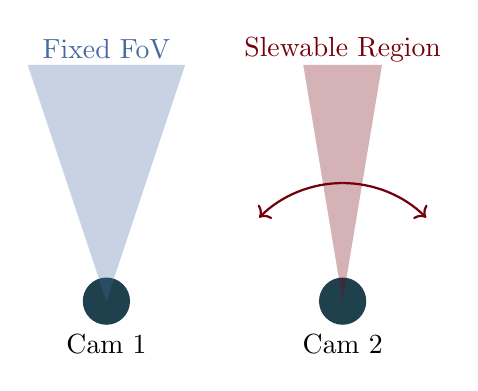
\begin{tikzpicture}
    % Cameras
    \fill[CDark] (-1.5, 0) circle (0.3);
    \fill[CDark] (1.5, 0) circle (0.3);
    
    % FoV 1 (Fixed)
    \fill[CBlue, opacity=0.3] (-1.5, 0) -- (-0.5, 3) -- (-2.5, 3) -- cycle;
    \node[CBlue] at (-1.5, 3.2) {Fixed FoV};
    
    % FoV 2 (Slewable)
    \fill[Garnet, opacity=0.3] (1.5, 0) -- (2.0, 3) -- (1.0, 3) -- cycle;
    \draw[->, Garnet, thick] (1.5, 1.5) arc (90:45:1.5);
    \draw[->, Garnet, thick] (1.5, 1.5) arc (90:135:1.5);
    \node[Garnet] at (1.5, 3.2) {Slewable Region};
    
    % Labels
    \node[below] at (-1.5, -0.3) {Cam 1};
    \node[below] at (1.5, -0.3) {Cam 2};
\end{tikzpicture}

\end{document}
